\subsection{Proposed Approach for Generating Midcurve}
In previous chapters it is seen that the proposed midsurface computation approach, first simplifies the input model by defeaturing, unifies the feature representation by generalization and then decomposes the simplified model into cells. Cellular topology makes devising generic approach for computing midsurface, easier and deterministic. Similar approach can also be used in computing midcurve from a profile.

Following is the proposed approach for computing midcurve which takes the input profile though similar stages as that of computation of midsurface. 
 
 %%\bigskip

\begin{figure}[h]
\centering 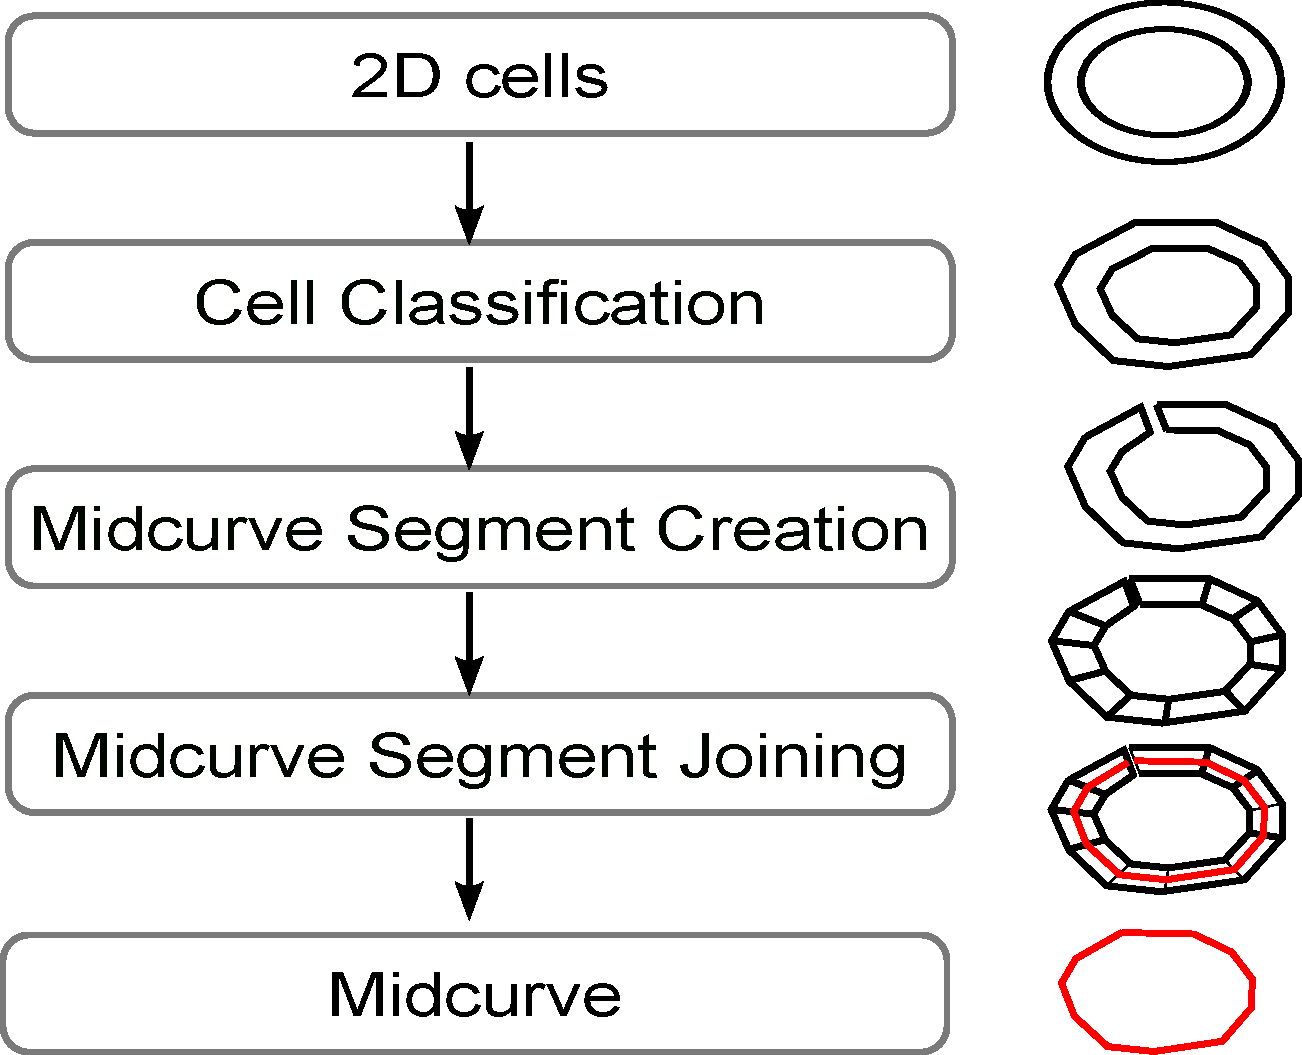
\includegraphics[width=0.5\linewidth]{../Common/images/SystemArchitectureMidcurve_2.pdf} 
\caption{Overall Wokflow of Proposed Midcurve Computation}
\label{fig_sysarchmidcurve}
\end{figure}

%%\bigskip

Figure~\ref{fig_sysarchmidcurve} shows the stages which are explained below:

\begin{enumerate} [noitemsep,topsep=2pt,parsep=2pt,partopsep=2pt]
\item Input to this approach is a profile, of a generalized Loft of $\mathcal{ABLE}$ paradigm, who is an owner feature of a $sCell$ for which a midsurface patch is being computed. The profile is typically made up of a variety of curves, such as lines, arcs, splines, etc. joined end-to-end forming closed loops. 
\item During simplification of the profile, the curves are faceted into linear segments. Thus the input profile becomes a polygon. This is termed as ``Polygonization''.
\item Polygon decomposition approach needs a single polygon whereas Loft feature's sketch may have inner profiles representing holes. These inner profiles are connected to outer boundary profile via bridge curves. Thus multiple profiles get converted to single continuous polygon. This is termed as ``Unification''.
\item During decomposition the polygon is split into sub-polygons, called 2D cells.
\item The set of connected 2D cells is used to compute the midcurve.
\end{enumerate}

Amongst the stages shown, Polygonization and Unification are already established techniques. Decomposition and Midcurve Computation are the two areas in which the present research work has contributed. Following subsections elaborate them in details. Input to them is a polygon which is arrived at after the``Polygonization'' and ``Unification'' processes,as  mentioned above. %Thus, the polygon is used as input to the further stages.

% the process of computing a midcurve goes through two phases viz. Decomposition and Midcurve computation. The process of polygon decomposition devised here, is based on an algorithm originally developed by Mark Bayazit~\cite{Bayazit}. He mentions basic rules for decomposition as:
%\begin{enumerate} [noitemsep,topsep=2pt,parsep=2pt,partopsep=2pt]
%\item A polygon can be broken into convex regions by eliminating all reflex vertices.
%\item A reflex vertex can only be removed if the diagonal connecting to it is within the range given by extending its neighboring edges; otherwise, its angle is only reduced.
%\end{enumerate}
%


\subsection{Polygon Decomposition}

Polygon decomposition is the partitioning of polygons into primitive sub-polygons. 
%Polygons come with different types of variations. They can be simple or self-intersecting, with or without holes, concave or convex etc. Although the algorithms presented here can compute midcurves for any simple polygon, but they are most relevant for thin elongated shapes such as alphabets made using Ribbon-like primitives. %For this work, more focus is given on profiles with constant thickness with test cases based on English alphabets. 
Strategy for `where-to-partition' depends on the application's need. Decompositions are done in such a way that minimum number of convex sub-polygons produced or total length of the boundary is minimized, etc. Convex Partitioning is one of the most popular method of polygon decomposition where partitioning happens at vertices having concave angle. Thus, as the concavity at those vertices is removed, after partitioning, the sub-polygons generated are of convex type having all vertices with convex angle. 

 %%\bigskip

\begin{figure}[h]
\centering 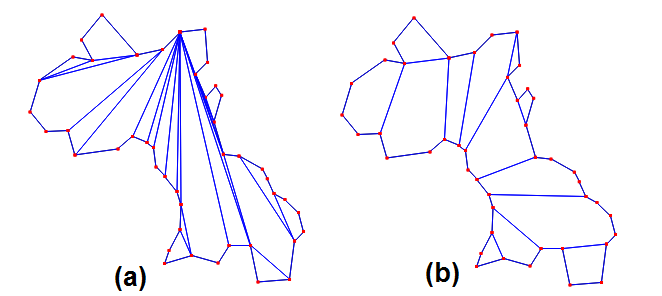
\includegraphics[width=0.62\linewidth]{../Common/images/convexcgal} 
\caption{Convex Partitioning (Source: CGAL~\cite{cgal})}
\label{fig_cgal}
\end{figure}

%%\bigskip

Figure~\ref{fig_cgal}a shows one of the possible polygon decomposition approaches whereas Figure~\ref{fig_cgal}b shows Convex Partitioning. The present research proposes to go in the direction of Convex partitioning but with an enhanced approach as elaborated below.

%Within the minimum component criterion, the methods are further classified based on whether or not Steiner points (brand new, non polygonal vertices) are allowed. A method devised here is of a convex-partitioning type with Steiner points allowed.   

The objective of polygon decomposition by convex partitioning method, is to remove `'concavity'' of the polygon. Figure~\ref{fig_concave} shows examples of concave and convex polygons with a simple line test. 


 %%\bigskip

\begin{figure}[h]
\centering 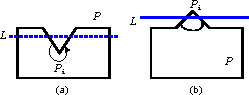
\includegraphics[width=0.62\linewidth]{../Common/images/polyconcavity.pdf} 
\caption{Concave and Convex Polygon}
\label{fig_concave}
\end{figure}

%%\bigskip

A polygon with any of the internal angles greater than 180 degrees is known as a concave polygon. As seen in Figure~\ref{fig_concave}a, if a line ($L$) passing through the polygon ($P$) cuts more than two places then its a concave polygon. This is due to $>180$ angle at vertex $P_i$. Such vertices are known as Reflex or Concave vertices and their presence is termed as ``concavity'' of the polygon. Figure~\ref{fig_concave}b shows a case where $L$ cuts $P$ only at two places. It is a convex polygon. It is so due to all vertices having angles $<180$. All such vertices are termed as convex vertices.

The objective of Convex Partitioning is to remove ``concavity'' of the polygon. Figure~\ref{fig_LienCEP}a shows the overall process. Concavity of the polygon $P$ is computed by detecting reflex vertices. Polygon is decomposed such that at-least one reflex vertex ($r$) is turned into convex vertex. If such vertex is found, $P$ gets decomposed into two sub-polygons $P_1, P_2$. Each of them goes through the same process as original $P$, till concavity of all the (sub)polygons is removed. Figure~\ref{fig_LienCEP}b shows how the recursive decomposing takes place.


 %%\bigskip

\begin{figure}[h]
\centering 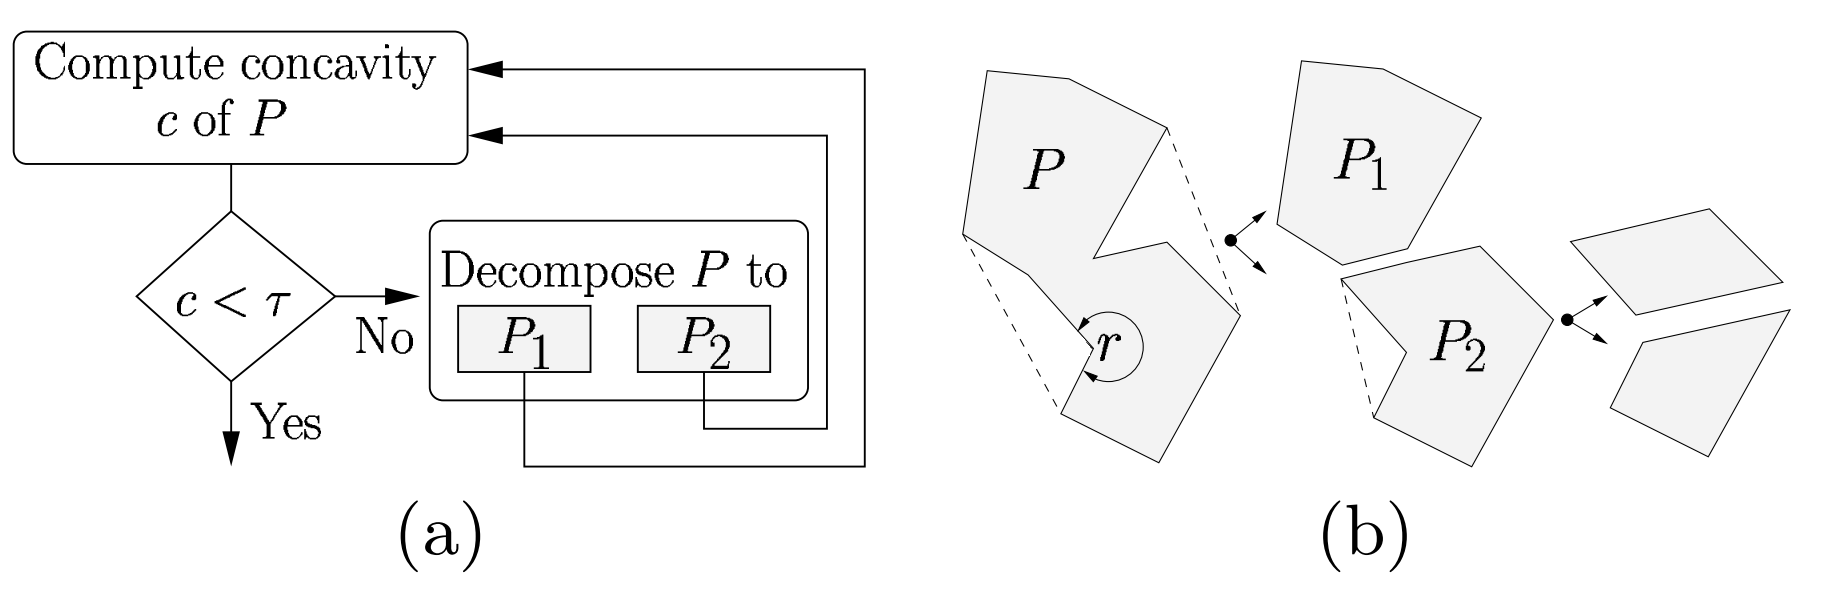
\includegraphics[width=0.92\linewidth]{../Common/images/LienCEP} 
\caption{Convex Partitioning by Recursion (Source: Lien~\cite{Lien2004})}
\label{fig_LienCEP}
\end{figure}

%%\bigskip

Polygon decomposition algorithm proposed in the present research work is based on existing convex partitioning method presented by Bayazit~\cite{Bayazit}. 

Following are the steps of the existing approach. Enhancements done to it are explained in the end.  The comparison between Bayazit's approach and the present research approach is also presented.

%%\subsubsubsection{Theoretical Background}

%%\begin{enumerate}
%%[noitemsep,topsep=2pt,parsep=2pt,partopsep=2pt]
%%%\begin{list}{}{}
%%\item {\bf Polygon}: A polygon $P$ of $n$ vertices is defined as 
%%
%%$P = \{P_0,P_1,...,P_{n-1}\}$
%%
%%where, the vertices are in counter clockwise (ccw) order. Polygon $P$ can also be defined in terms of a set of connected edges as  
%%
%%$P = \{\overline{P_0 P_1},\overline{P_1 P_2}...,\overline{P_{n-1} P_0}\}$
%%
%%In case of shapes which have non-linear elements, they are faceted and brought in terms of connected lines.
%%
%%\item {\bf Simple}: A polygon is simple if none of the edges intersect other edges anywhere else other than the shared endpoints of adjacent edges.
%%\begin{displaymath}
%%\forall \quad \overline{P_i P_j}, \overline{P_k P_l} \in P, \left\{ 
%%  \begin{array}{l l}
%%     \overline{P_i P_j} \cap \overline{P_k P_l} = \phi , j \neq k\\
%%     \overline{P_i P_j} \cap \overline{P_k P_l} = P_k  , j = k
%%  \end{array} \right.
%%\end{displaymath}
%%
%%\item {\bf Diagonal}: $\overline{P_i P_k}$ is a {\em diagonal} of $P$.  In other words, a {\em diagonal} is just a line segment between two vertices that only touches the interior of the polygon.
%%
%%\item {\bf Area}: $Area$ formed by three vertices in order ($ P_{j-1}, P_j,  P_{j+1}$) or two consecutive {\em edges} ($ \overline{P_{j-1} P_j} \cap \overline{P_j P_{j+1}}$ ) is a signed quantity which is given by
%%\begin{displaymath}
%%\begin{array}{l l}
%%Area = P_{j-1}.X ( P_j.Y - P_{j+1}.Y) + \\
%%P_j.X (P_{j+1}.Y -  P_{j-1}.Y) + \\
%%P_{j+1}.X ( P_{j-1}.Y - P_j.Y) 
%% \end{array} 
%%\end{displaymath}
%%
%%\item {\bf Left}: $P_{j+1}$ is {\em Left} of $ \overline{P_{j-1} P_j}$ if $Area( P_{j-1}, P_j,  P_{j+1}) > 0$ 
%%
%%\item {\bf Right}: $P_{j+1}$ is {\em Right} of $ \overline{P_{j-1} P_j}$ if $Area( P_{j-1}, P_j,  P_{j+1}) < 0$ 
%%
%%\item {\bf Collinear}: $P_{j+1}$ is {\em Collinear} with $ \overline{P_{j-1} P_j}$ if $Area( P_{j-1}, P_j,  P_{j+1}) = 0$ 
%%
%%\item {\bf Reflex}: Let  $ P_{j-1}, P_j,  P_{j+1} \in P $ , if the interior $\angle P_{j-1}, P_j,  P_{j+1}$ is greater than $\pi$  then $P_j$  is a concave or {\em reflex} vertex. $Area < 0$
%%
%%\item {\bf Intersect}: For  $\overline{P_i P_j}$ to intersect $\overline{P_k P_l}$, either of $P_k, P_l$ should be on {\em Left} of  $\overline{P_i P_j}$ and the other vertex should be on {\em Right}. Intersection could be of {\em Line} type where extended intersection can be calculated or of {\em Segment} type where only internal (within the range of either of the segments, $\overline{P_i P_j}$ or $\overline{P_k P_l}$) intersections are returned.
%%
%%\item {\bf Visibility/Can-See}: $P_k$ is visible from $P_i$ if $\overline{P_i P_k}$ is a {\em diagonal} of $P$. 
%%
%%%\end{list}
%%\end{enumerate}

%%\subsubsubsection{Steps to Decompose Polygon}

%%Let $P$ be a simple polygon.  The Partitioning of $P$ is defined by the decomposition of $P$ into partitions of non-overlapping sub-polygons by adding internal {\em diagonals} between vertices  $P_i$ or by adding new (Steiner) vertices on {\em edges} $\overline{P_i P_j}$. Partitioning is continued till all possible cuts are made. Steps are as follows:

Steps to decompose a polygon are:

\def\polygondecompositionstepsfigs{0.2}
%\begin{tabular}[h]{@{}p{5cm}  p{3cm}@{}}
\begin{enumerate}
[noitemsep,topsep=2pt,parsep=2pt,partopsep=2pt,leftmargin=*]
%\begin{list}{}{}

%------------------------------------------------------------------------------------------------------------------------------------
\item 
Input is a simple polygon, denoted by $P$. It is defined as a list of vertices $P_i$ (where, $i=1 \rightarrow n$) ordered in a counter-clockwise manner. So, 
$P = \{P_0,P_1,...,P_{n-1}\}$

Polygon $P$ can also be defined in terms of a set of connected edges, as:

$P = \{\overline{P_0 P_1},\overline{P_1 P_2}...,\overline{P_{n-1} P_0}\}$

A polygon is simple if none of the edges intersect other edges anywhere-else other than at the shared endpoints of adjacent edges. This condition is denoted as:

\begin{displaymath}
\forall \quad \overline{P_i P_j}, \overline{P_k P_l} \in P, \left\{ 
  \begin{array}{l l}
     \overline{P_i P_j} \cap \overline{P_k P_l} = \phi , j \neq k\\
     \overline{P_i P_j} \cap \overline{P_k P_l} = P_k  , j = k
  \end{array} \right.
\end{displaymath}

\item All the vertices of the polygon are iterated one by one in counter-clockwise manner. %&

 %%\bigskip

\begin{figure}[h]
\centering 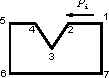
\includegraphics[width=0.33\linewidth]{../Common/images/polydecomp_traverse_1.pdf} 
\caption{Polygon Traversal}
\label{fig_traverse}
\end{figure}

%%\bigskip

Figure~\ref{fig_traverse} shows simple polygon with 7 vertices, ordered counterclockwise. The current vertex is set as $P_i$  and the direction of traversal is shown by the arrow.

%------------------------------------------------------------------------------------------------------------------------------------
\item 
$P_i$ is checked if it is a reflex vertex by measuring angle $r$.

 %%\bigskip

\begin{figure}[h]
\centering 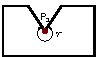
\includegraphics[width=0.3\linewidth]{../Common/images/polydecomp_reflex_1.pdf} 
\caption{Polygon Reflex Vertex Detection}
\label{fig_reflex}
\end{figure}

%%\bigskip

Figure~\ref{fig_reflex} shows that $P_3$ is reflex, as per definition below:

Let  $ P_{j-1}, P_j,  P_{j+1} \in P $ , if the interior $\angle P_{j-1}, P_j,  P_{j+1}$ is greater than $\pi$  then $P_j$  is a concave or {\em reflex} vertex.

Another way to test reflexivity or concavity of a vertex is if $Area < 0$, where $Area$ is a signed quantity and is as defined below:

$Area$ formed by three vertices in order ($ P_{j-1}, P_j,  P_{j+1}$) or two consecutive {\em edges} ($ \overline{P_{j-1} P_j} \cap \overline{P_j P_{j+1}}$ ) is a signed quantity which is given by:

\begin{displaymath}
\begin{array}{l l}
Area = P_{j-1}.X ( P_j.Y - P_{j+1}.Y) + \\
P_j.X (P_{j+1}.Y -  P_{j-1}.Y) + \\
P_{j+1}.X ( P_{j-1}.Y - P_j.Y) 
 \end{array} 
\end{displaymath}

$P_3$ being a reflex vertex is termed as $R$.

%------------------------------------------------------------------------------------------------------------------------------------
\item 
Objective is to decompose the polygon at $R$ such that its concavity is removed and the two sub-polygons that get created will have convex angles at respective vertices which originally was $R$. So, for cutting the concave angle at $R$, lines incident at it are extended. The piece of polygon in between the intersection of extended lines is called as ``Range''. 

 %%\bigskip

\begin{figure}[h]
\centering 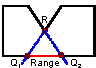
\includegraphics[width=0.3\linewidth]{../Common/images/polydecomp_range_1.pdf} 
\caption{Range Detection}
\label{fig_range}
\end{figure}

%%\bigskip

Figure~\ref{fig_range} shows that $R$ is the reflex vertex. Lines incident at it, i.e. the line coming into $P_i$ and going out of $P_i$, are extended till they intersect remaining of the Polygon, say at $Q_1$ and $Q_2$. The segment within $Q_1$ and $Q_2$ is called $Range$.%&

%------------------------------------------------------------------------------------------------------------------------------------
\item 

Now the intent is to find a vertex so that line from $R$ to it can be used for partitioning the polygon. Following are the cases depending on the number and types of vertices found in the $Range$.

\begin{enumerate}
[noitemsep,topsep=2pt,parsep=2pt,partopsep=2pt,leftmargin=*]

\item {\bf None}: If there are no vertices found in the range, or any of the polygon vertices themselves are end vertices of the range then a new vertex is created in the middle of $Range$. This new vertex is called as ``Steiner'' vertex.

 %%\bigskip

\begin{figure}[h]
\centering 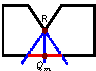
\includegraphics[width=0.3\linewidth]{../Common/images/polydecomp_mid_1.pdf} 
\caption{Steiner Vertex Creation}
\label{fig_mid}
\end{figure}

%%\bigskip

Figure~\ref{fig_mid} shows that there are no vertices in the $Range$ so a Steiner vertex $Q_m$ is created and thus line $R-Q_m$ becomes the cutting or partitioning line, called ``chord'', used to split the polygon.

\item {\bf Closest Reflex}: If there are multiple reflex vertices in the $Range$ then the closest amongst them gets the highest priority to form the chord.

\item {\bf Reflex}: If a vertex found in the $Range$ is a sole reflex vertex then its gets the next priority to form the chord.

\item {\bf Closest}: If non of the vertices found in the $Ranges$ are reflex vertex, then closes amongst those gets the priority to form the chord.

 %%\bigskip

\begin{figure}[h]
\centering 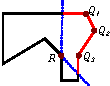
\includegraphics[width=0.3\linewidth]{../Common/images/polydecomp_choice_1.pdf} 
\caption{Vertex Priorities for Chord Creation}
\label{fig_choice}
\end{figure}

%%\bigskip

Figure~\ref{fig_choice} shows a different profile shape examples having 3 candidate vertices in the $Range$ to form the chord. $Q_3$ being the only reflex vertex, gets the chance to form the chord.

\item {\bf Visible}: It is made sure that the selected vertex $Q_3$ is ``visible'' from the reflex vertex $R$. If it is not so, then this cut can not be made. The next best choice is chosen for evaluation. Visibility test is performed as defined below:

$P_k$ is visible from $P_i$ if $\overline{P_i P_k}$ is a {\em diagonal} of $P$. 

where, ``Diagonal'' is defined as: $\overline{P_i P_k}$ is a {\em diagonal} of $P$.  So, a {\em diagonal} is a line segment between two vertices that only touches the interior of the polygon.

\end{enumerate}

\item Polygon is divided at the chord. Figure~\ref{fig_divide} shows the formation of the chord between $R-Q_3$.

 %%\bigskip

\begin{figure}[h]
\centering 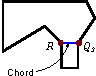
\includegraphics[width=0.28\linewidth]{../Common/images/polydecomp_divide_1.pdf} 
\caption{Polygon Decomposition by the Chord}
\label{fig_divide}
\end{figure}

%%\bigskip

%\end{tabular}

%------------------------------------------------------------------------------------------------------------------------------------
\item 
The decomposed sub-polygons are sent through the same process recursively till there are no reflex vertices left. 

\item  
Output of the above steps is a set of connected sub-polygons. 

%\end{list}
\end{enumerate}


%\subsubsubsection{Improvements over Bayazit's algorithm}

The proposed approach improves upon the Bayazit's algorithm~\cite{Bayazit} stated above, in terms of expanding search to include even the extreme vertices in the range, thereby giving minimal and elongated sub-polygon shapes. Midcurves are typically for thin, elongated shapes. Thus the proposed improvement results in the sub-polygons of shape characteristics needed for computation of midcurves.

Following is the list of salient improvements over  Bayazit's algorithm~\cite{Bayazit}:

\begin{enumerate}
[noitemsep,topsep=2pt,parsep=2pt,partopsep=2pt,leftmargin=*]

\item If there are any vertices at the ends of the $Range$, they were getting ignored, or were sent for ``None'' (i.e. Steiner vertex) case. The proposed approach includes them as candidates for further evaluation based on the priorities stated above.

%%\bigskip

\begin{figure}[h]
\centering 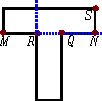
\includegraphics[width=0.25\linewidth]{../Common/images/polydecomp_mine_1.pdf} 
\caption{Including Extreme Range Vertices}
\label{fig_mine}
\end{figure}

%%\bigskip


Figure~\ref{fig_mine} shows that incoming edge ($MR$) is hitting the end vertices of the test-line ($QN$) or is collinear, it ($Q$) was getting ignored in the existing algorithm~\cite{Bayazit}. In that case the next closet vertex ($S$) was getting chosen. This was corrected in the proposed algorithm and a shorter cut with chord $RQ$ is done.

\item The midcurve creation algorithm requires these sub-polygons to be of two primitive types viz. triangles and quadrilaterals. So, if any of the sub-polygons has more than 4 sides then those sub-polygons are are triangulated with Constrained Delaunay Triangulation (CDT).

%%\bigskip

\begin{figure}[h]
\centering 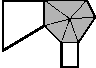
\includegraphics[width=0.3\linewidth]{../Common/images/polydecomp_divide_all_2.pdf} 
\caption{Triangulation of More Than 4 Sided Polygons}
\label{fig_divideall}
\end{figure}

%%\bigskip

Figure~\ref{fig_divideall} shows a sub-polygon with more than 4 sides has been triangulated.

\end{enumerate}

%\begin{tabular}[h]{@{}p{0.6\linewidth} p{0.03\linewidth} p{0.27\linewidth}@{}}
%
%If any incoming edge ($MR$) is hitting the end points of the test-line ($QN$) or is collinear, it ($Q$) was getting ignored in the existing algorithm~\cite{Bayazit}. In that case the next closet vertex ($S$) was getting chosen. This was corrected in the proposed algorithm and the shorter cut ($RQ$) is done.&&
%
%\raisebox{-.9\height}{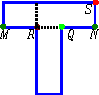
\includegraphics[width=0.6\linewidth]{..//Common/images/polydecomp_mine.pdf} }\\
%\\
%\end{tabular}

Algorithm~\ref{alg:midcurves:polygondecomposition} shows the proposed approach of polygon decomposition. 

\bigskip

\begin{algorithm}[H]
	\caption{Polygon Decomposition}
	\label{alg:midcurves:polygondecomposition}
	\begin{algorithmic}[1]
		\REQUIRE 2D Planar polygon represented by list of vertices
		\ENSURE Vertices in counter-clockwise direction

		\WHILE{End of vertices list has  not reached}
			\STATE Get the current vertex.
			\IF {current vertex is a Reflex vertex $R$}           
				\STATE Extend  the  edges incident at $R$ until they hit an edge

				\IF {Extension line and Polygon side are collinear} 				
					\STATE Find closest vertex which is not internal to the extension line
				\ENDIF

				\IF {there are no vertices to connect to}			
					\STATE choose a vertex in the middle
				\ELSE
					\STATE Find vertex to connect to
					\STATE Find best vertex $Q_i$ within the range, to form the partitioning chord
					\STATE Make sure $Q_i$ is visible from $R$
				\ENDIF
			\ENDIF
		\ENDWHILE
		\STATE  Split the polygon at the cutting chord (line $RQ_i$)
		%ADDED
		\STATE Repeat with sub-polygons till there are no reflex vertices left. 
		\STATE Triangulate polygons with more than 4 sides.
	\end{algorithmic}
\end{algorithm}

%%\bigskip

As the last step in the {\bf Algorithm \ref{alg:midcurves:polygondecomposition}} triangulates the remaining polygons, this algorithm guarantees presence of sub-polygons with 3 and 4 sides only. Further algorithms, like the one mentioned below {\bf Algorithm \ref{alg:midcurves:midcurvescreation}}, thus, needs to devise logic for only the triangles and quadrilaterals, making it less error prone and more deterministic. {\bf Table \ref{tbl:midcurves:partitioncomparision}} demonstrates improvements over Bayazit's~\cite{Bayazit} algorithm with examples.  


\def\partitioncomparisionraise{0.08}
\def\partitioncomparisionfig{0.98}

%%\bigskip

\begin{table}[!h]
\caption{Comparison of Proposed Polygon Decomposition Approach with the Existing One}
\begin{tabular}[h]{@{} p{0.31\linewidth} p{0.31\linewidth} p{0.31\linewidth}@{}}
\toprule



{\bf Input Polygonal Profile} & {\bf Bayazit's Approach} & {\bf Current Research Approach}\\
\midrule
%------------------------------------------------------------------------------------------------------------------------------------
%T &
\raisebox{\partitioncomparisionraise\height}{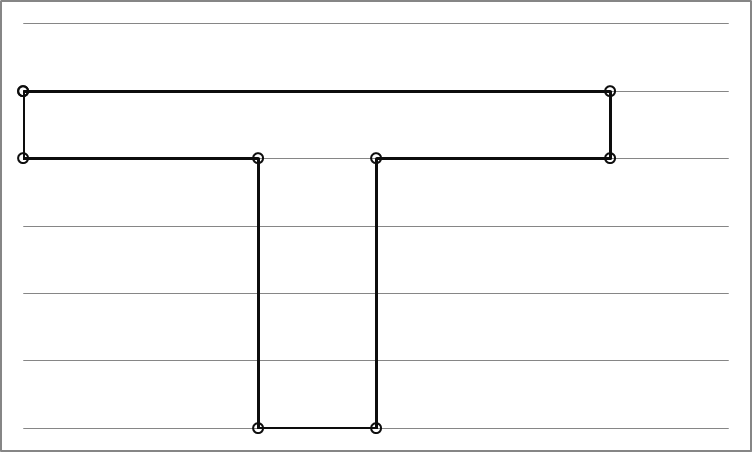
\includegraphics[width=\partitioncomparisionfig\linewidth]{..//Common/images/Ts.png}} &
\raisebox{\partitioncomparisionraise\height}{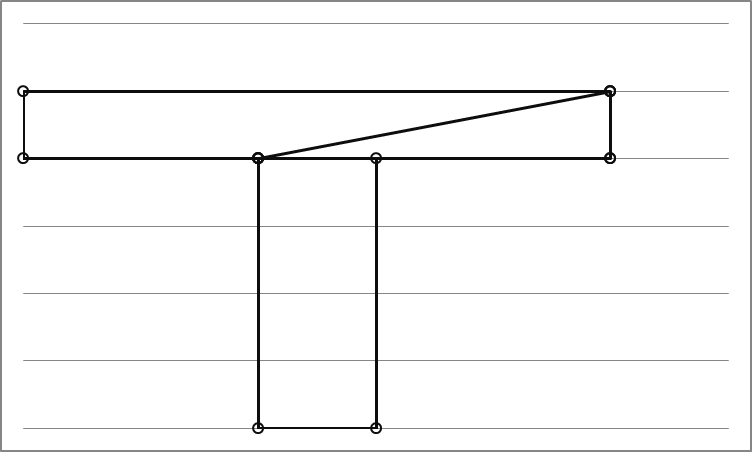
\includegraphics[width=\partitioncomparisionfig\linewidth]{..//Common/images/Tb.png}}&
\raisebox{\partitioncomparisionraise\height}{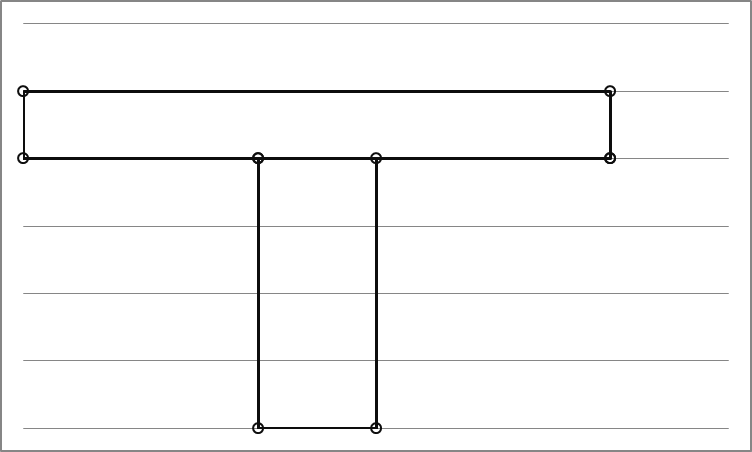
\includegraphics[width=\partitioncomparisionfig\linewidth]{..//Common/images/Tp.png}} \\


%------------------------------------------------------------------------------------------------------------------------------------
%Plus  &
\raisebox{\partitioncomparisionraise\height}{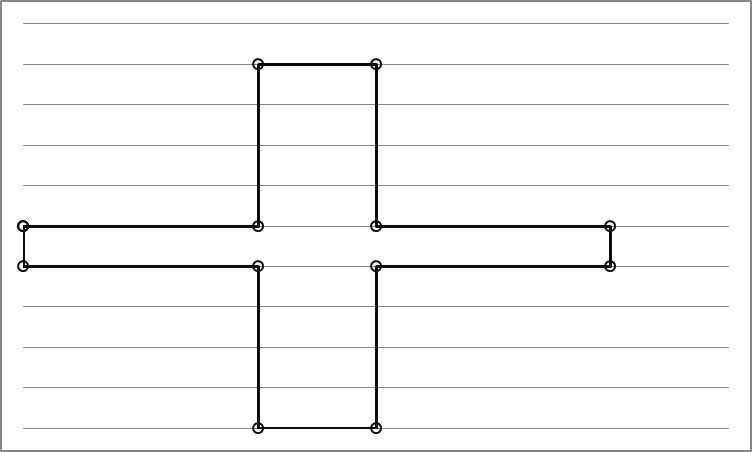
\includegraphics[width=\partitioncomparisionfig\linewidth]{..//Common/images/Pluss.png}} &
\raisebox{\partitioncomparisionraise\height}{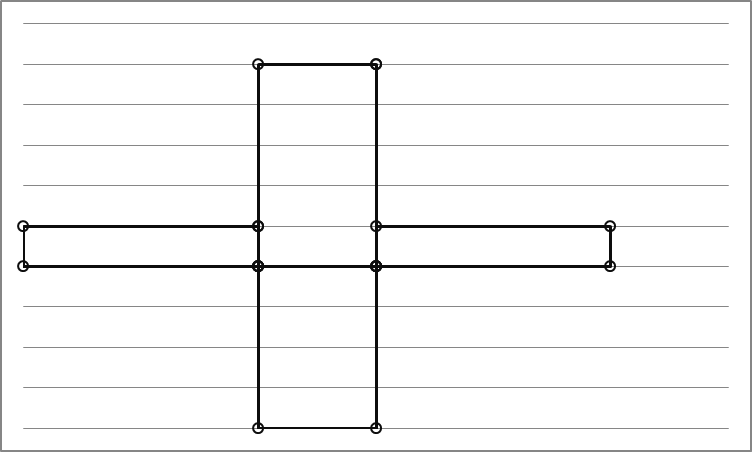
\includegraphics[width=\partitioncomparisionfig\linewidth]{..//Common/images/Plusb.png}}&
\raisebox{\partitioncomparisionraise\height}{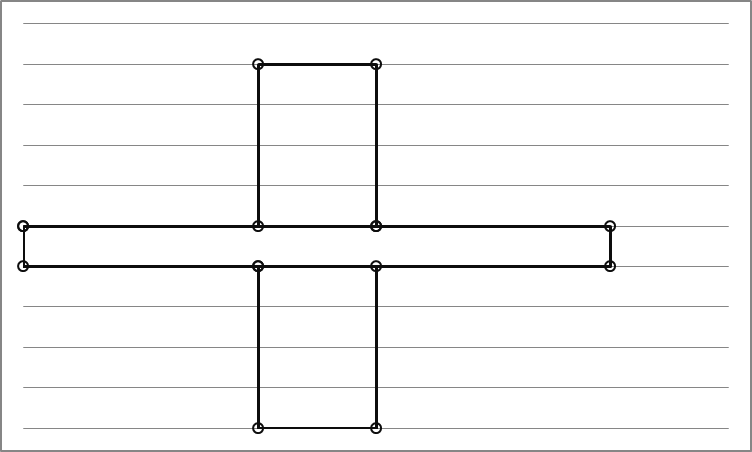
\includegraphics[width=\partitioncomparisionfig\linewidth]{..//Common/images/Plusp.png}} \\


%------------------------------------------------------------------------------------------------------------------------------------
%Star &
\raisebox{\partitioncomparisionraise\height}{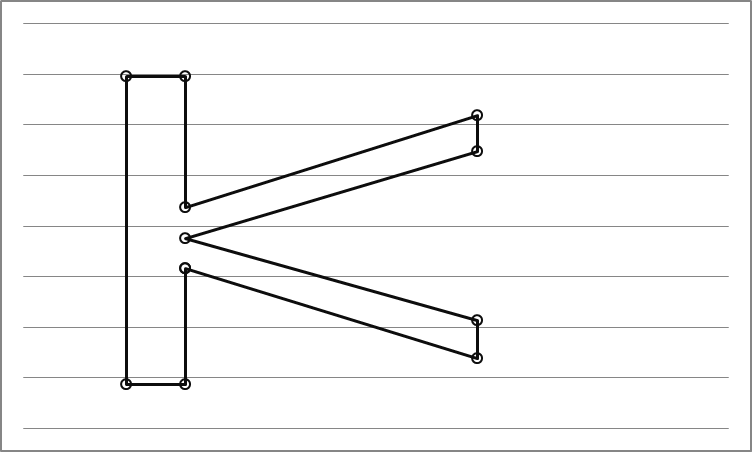
\includegraphics[width=\partitioncomparisionfig\linewidth]{..//Common/images/Ks.png}} &
\raisebox{\partitioncomparisionraise\height}{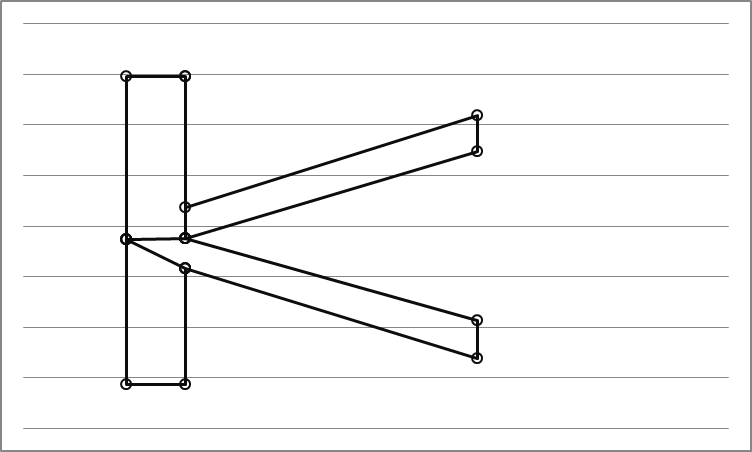
\includegraphics[width=\partitioncomparisionfig\linewidth]{..//Common/images/Kb.png}}&
\raisebox{\partitioncomparisionraise\height}{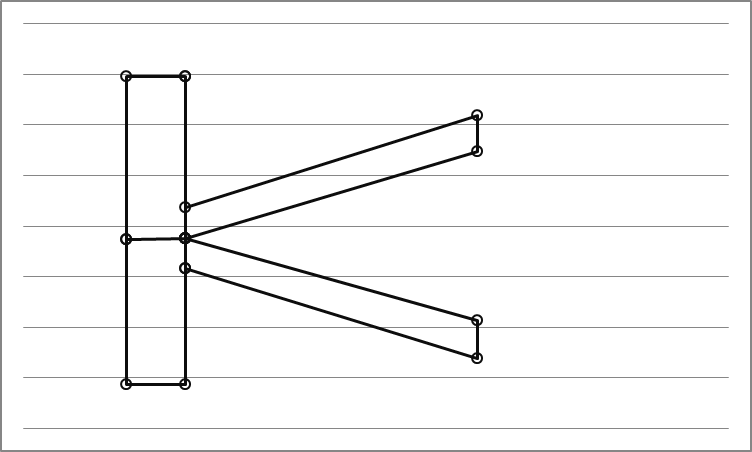
\includegraphics[width=\partitioncomparisionfig\linewidth]{..//Common/images/Kp.png}} \\

%------------------------------------------------------------------------------------------------------------------------------------
%Star &
\raisebox{\partitioncomparisionraise\height}{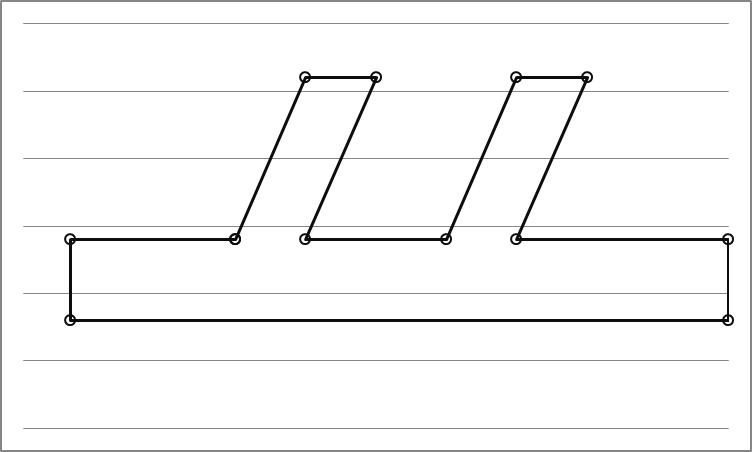
\includegraphics[width=\partitioncomparisionfig\linewidth]{..//Common/images/DoubleKs.png}} &
\raisebox{\partitioncomparisionraise\height}{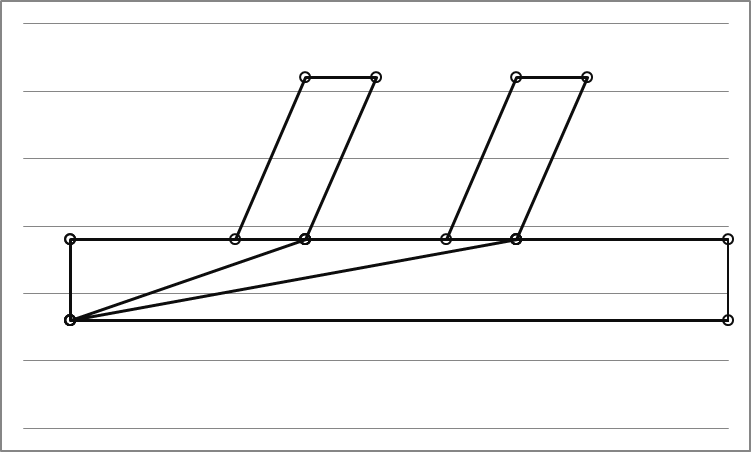
\includegraphics[width=\partitioncomparisionfig\linewidth]{..//Common/images/DoubleKb.png}}&
\raisebox{\partitioncomparisionraise\height}{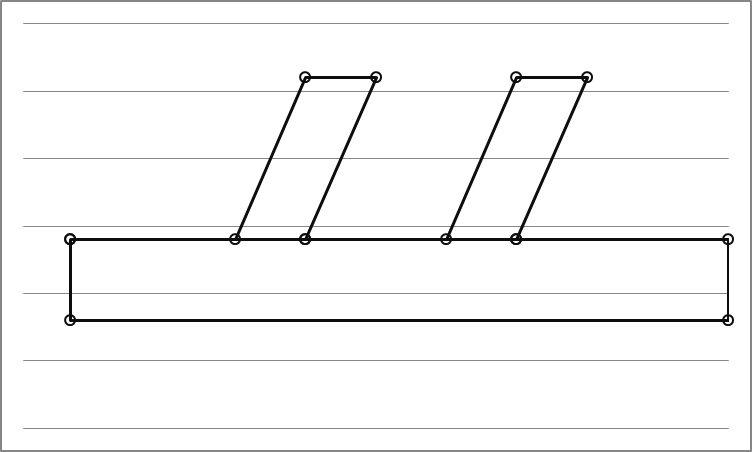
\includegraphics[width=\partitioncomparisionfig\linewidth]{..//Common/images/DoubleKp.png}} \\

%\bottomrule
\end{tabular}
\label{tbl:midcurves:partitioncomparision}
\end{table}

Table~\ref{tbl:midcurves:partitioncomparision} shows comparison of results of polygon decomposition between the existing Bayazit's~\cite{Bayazit} approach and the approach proposed in the present research work. The output of the proposed approach has primitives of types triangles and quadrilaterals and no other redundant splittings. The resulting sub-polygons are sent for computing connected midcurves, as described in the following section.


\subsection{Generation of Midcurves from Sub-Polygons}

The objective of this module is to compute a connected midcurve from the set of sub-polygons received from the previous module.
%The proposed approach is similar to what has been proposed for midsurface creation from solid cells. The polygon decomposition mentioned before is a cellular decomposition in the context of polygons and the sub-polygons generated are 2D cells. 
Following is the proposed approach of generating midcurve from 2D cells.

 %%\bigskip

%\begin{figure}[h]
%\centering 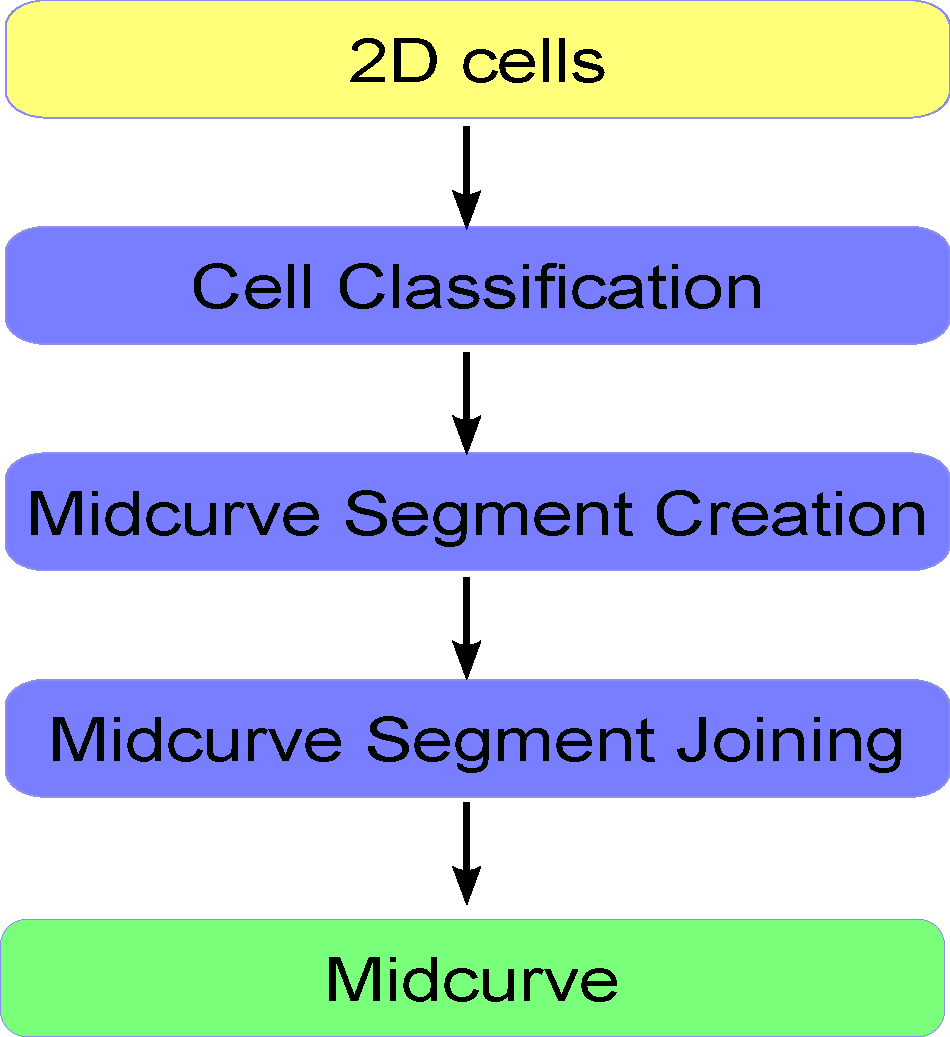
\includegraphics[width=0.5\linewidth]{../Common/images/SystemArchitectureMidcurve_1.pdf} 
%\caption{Proposed Midcurve Computation after Decomposition}
%\label{fig_midcurvedecomp}
%\end{figure}

%%\bigskip

Figure~\ref{fig_sysarchmidcurve} shows the stages which are explained below:

\begin{enumerate} [noitemsep,topsep=2pt,parsep=2pt,partopsep=2pt]
\item Set of 2D cells (sub-polygons) is the input. They are of only two types Triangles and Quadrilaterals. 
\item Cells are classified into different classes based on type, i.e. triangle or quadrilateral and on the number of sides which are chords. A chord is a common interface-boundary shared between two cells. Each chord will have two sides owned by two different cells. 

%%\bigskip

\begin{figure}[h]
\centering 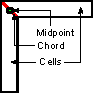
\includegraphics[width=0.25\linewidth]{../Common/images/midcurve_polydecomp_2.pdf} 
\caption{Chord Midpoint as Location for Joining Midcurve Segments}
\label{fig_midcurvechords}
\end{figure}

%%\bigskip

Figure~\ref{fig_midcurvechords} shows ``L'' shaped profile with 2 quadrilateral shaped cells, with a chord at the interface and its midpoint. Following steps make sure that midcurve patches from both sides of the chord are joined at the midpoint of the chord.
\item Midcurve segments are created based on the particular class of cells, elaborated in Tables~\ref{tbl:midcurves:trianglecases},~\ref{tbl:midcurves:polygoncases}. `Thinness' is an important criterion in choosing midcurves for the individual shape. Midcurves are generated along longer-length and not across shorter width.

%%\bigskip

\begin{figure}[h]
\centering 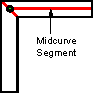
\includegraphics[width=0.25\linewidth]{../Common/images/midcurve_polymid_2.pdf} 
\caption{Midcurve Segment Creation}
\label{fig_polymid}
\end{figure}

%%\bigskip

Figure~\ref{fig_polymid} shows midcurve segment computed for one of the cells. In shapes like 'L' midcurves from both sub-polygons, across the chord, join together at a vertex, naturally. Additional extensions are not required.

\item Midcurve patches are joined in cases where there is gap.

%%\bigskip

\begin{figure}[h]
\centering 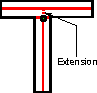
\includegraphics[width=0.25\linewidth]{../Common/images/midcurve_extend_2.pdf} 
\caption{Midcurve Segment Extension}
\label{fig_extend}
\end{figure}

%%\bigskip

Figure~\ref{fig_extend} shows  'T' shaped polygon. The horizontal midcurve does not connect with the common chord. In this case one of the midcurves is extended to join the other. 

\item Output is a well-connected midcurve.
\end{enumerate}

Following tables detail various cases and the process to compute midcurve segments.

\def\trianglecasestablewidth{0.45}

\bigskip

\begin{table}[!h]
\caption{Triangle Cases of Midcurve Configuration}
\label{tbl:midcurves:trianglecases}
\begin{tabular}[h]{@{}p{0.15\linewidth}@{} p{0.18\linewidth} @{}p{0.5\linewidth} p{0.15\linewidth}@{}} \toprule
{\bf Shape } & {\bf Chords }  & {\bf Rule} & {\bf Diagram}\\
\midrule

%------------------------------------------------------------------------------------------------------------------------------------
Triangle &
None&
No Midcurve &
\raisebox{-.9\height}{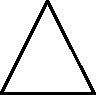
\includegraphics[width=\trianglecasestablewidth\linewidth]{..//Common/images/mids_t0.pdf} }\\

%------------------------------------------------------------------------------------------------------------------------------------
&
One &
Join Midpoint of the shorter side &
\raisebox{-.9\height}{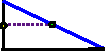
\includegraphics[width=\trianglecasestablewidth\linewidth]{..//Common/images/mids_t1_side.pdf} }\\

%------------------------------------------------------------------------------------------------------------------------------------
&
One &
Join Opposite vertex if both sides are of similar length &
\raisebox{-.9\height}{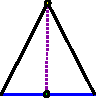
\includegraphics[width=\trianglecasestablewidth\linewidth]{..//Common/images/mids_t1.pdf} }\\

%------------------------------------------------------------------------------------------------------------------------------------
&
Two &
Join bisectors &
\raisebox{-.9\height}{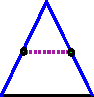
\includegraphics[width=\trianglecasestablewidth\linewidth]{..//Common/images/mids_t2.pdf} }\\

%------------------------------------------------------------------------------------------------------------------------------------
&
Three &
Join to centroid &
\raisebox{-.9\height}{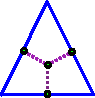
\includegraphics[width=\trianglecasestablewidth\linewidth]{..//Common/images/mids_t3.pdf} }\\

\bottomrule

\end{tabular}
\end{table}

\bigskip

\begin{table}[!h]
\caption{Quadrilateral Cases of Midcurve Configuration}
\label{tbl:midcurves:polygoncases}
\begin{tabular}[h]{@{}p{0.15\linewidth}@{} p{0.18\linewidth} @{}p{0.5\linewidth} p{0.15\linewidth}@{}} \toprule

{\bf Shape } & {\bf Chords }  & {\bf Rule} & {\bf Diagram}\\
\midrule
%------------------------------------------------------------------------------------------------------------------------------------
Quadrilateral &
None&
Find shortest side and create Midcurve in the direction average of both the adjacent sides &
\raisebox{-.9\height}{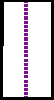
\includegraphics[width=\trianglecasestablewidth\linewidth]{..//Common/images/mids_q0.pdf} }\\

%------------------------------------------------------------------------------------------------------------------------------------
&
One (Shorter) &
Create Midcurve in the direction average of both the adjacent sides &
\raisebox{-.9\height}{
\includegraphics[width=\trianglecasestablewidth\linewidth]{..//Common/images/mids_q1s.pdf} }\\


%------------------------------------------------------------------------------------------------------------------------------------
&
One (Longer)&
Extend from Chord on longer side upto the midcurve &
\raisebox{-.9\height}{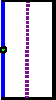
\includegraphics[width=\trianglecasestablewidth\linewidth]{..//Common/images/mids_q1l.pdf} }\\


%------------------------------------------------------------------------------------------------------------------------------------
&
Two (Opposite)&
Join midpoints &
\raisebox{-.9\height}{
\includegraphics[width=\trianglecasestablewidth\linewidth]{..//Common/images/mids_q2o.pdf} }\\


%------------------------------------------------------------------------------------------------------------------------------------
&
Two (Adjacent) &
Ignore the chord on longer side and use one-chord rule &
\raisebox{-.9\height}{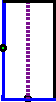
\includegraphics[width=\trianglecasestablewidth\linewidth]{..//Common/images/mids_q2a.pdf} }\\


%------------------------------------------------------------------------------------------------------------------------------------
&
Three &
Join to centroid &
\raisebox{-.9\height}{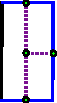
\includegraphics[width=\trianglecasestablewidth\linewidth]{..//Common/images/mids_q3.pdf} }\\


%------------------------------------------------------------------------------------------------------------------------------------
&
Four &
Join to centroid &
\raisebox{-.9\height}{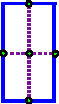
\includegraphics[width=\trianglecasestablewidth\linewidth]{..//Common/images/mids_q4.pdf} }\\

%\end{tabular}
%\label{Configurationsq}
%\end{table}
%
%\begin{table}[!h]
%\caption{Polygon cases of Midcurve configuration}
%\begin{tabular}[h]{|p{1cm} | p{1cm} | p{3cm} | p{1.2cm}|}
%\hline
%{\bf Shape } & {\bf Chords }  & {\bf Rule} & {\bf Diagram}\\
%\hline
%%
%%%------------------------------------------------------------------------------------------------------------------------------------
%%Polygon &
%%None&
%%If Thin, then CDT and CAT &
%%\raisebox{-.9\height}{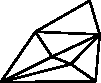
\includegraphics[width=\trianglecasestablewidth\linewidth]{..//Common/images/mids_p0.pdf} }\\
%%
%%%------------------------------------------------------------------------------------------------------------------------------------
%%&
%%Any &
%%Join to centroid &
%%\raisebox{-.9\height}{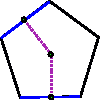
\includegraphics[width=\trianglecasestablewidth\linewidth]{..//Common/images/mids_pany.pdf} }\\
\bottomrule

\end{tabular}
\end{table}

\bigskip

Algorithm \ref{alg:midcurves:midcurvescreation} presents the proposed approach for midcurve computation from 2D cells in a pseudo-code format.

\bigskip

\begin{algorithm}[H]
	\caption{Midcurves Creation}
	\label{alg:midcurves:midcurvescreation}
	\begin{algorithmic}[1]
		\REQUIRE List of partitioned 2D Planar polygons represented by list of vertices in counter-clockwise direction
		\STATE Find internal-common edges called chords
		\STATE Iterate over all polygons and create chords at Full or Partial overlap
		\WHILE{End of Polygons list has  not reached}
			\STATE Get the current polygon $P$
			\STATE Get chords which are part of $P$
			\STATE Look at various configurations due to Num Sides and Num Chords
			\STATE Generate Midcurves
			\STATE Assign Midcurves on relevant side of the chord
		\ENDWHILE
		\STATE Extend chords which are not connected with other neighboring chords
	\end{algorithmic}
\end{algorithm}

\bigskip

Table~\ref{tbl:midcurves:connectingmidcurves} presents various cases demonstrating working of both, polygon decomposition as well as midcurve computation. It clearly demonstrates that the midcurve generated is well connected and represents the input profile shape faithfully.

\bigskip

\begin{table}[!h]
\caption{Partitions and Medial Computation}
\label{tbl:midcurves:connectingmidcurves}
\begin{tabular}[h]{@{} p{0.31\linewidth} p{0.31\linewidth} p{0.31\linewidth}@{}}
\toprule
{\bf Shape } & {\bf Partitions} & {\bf Midcurves}\\
\midrule
%------------------------------------------------------------------------------------------------------------------------------------
%L &
\raisebox{\partitioncomparisionraise\height}{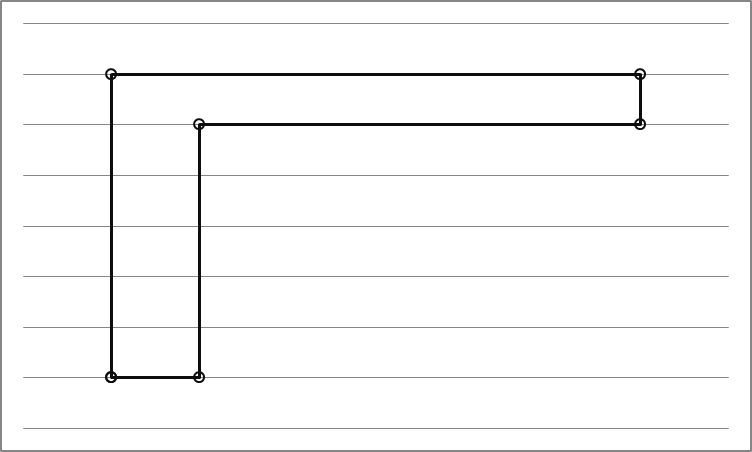
\includegraphics[width=\partitioncomparisionfig\linewidth]{..//Common/images/Ls.png}} &
\raisebox{\partitioncomparisionraise\height}{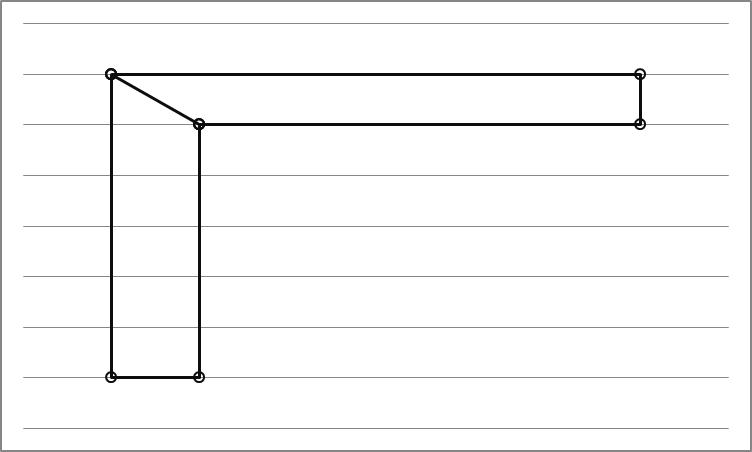
\includegraphics[width=\partitioncomparisionfig\linewidth]{..//Common/images/Lp.png}}&
\raisebox{\partitioncomparisionraise\height}{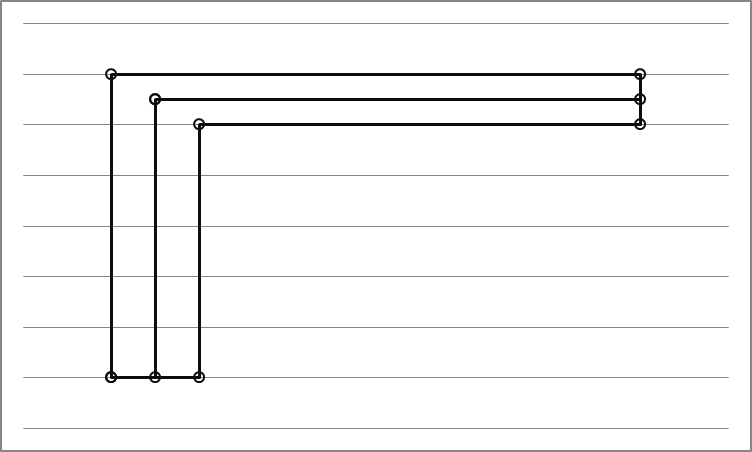
\includegraphics[width=\partitioncomparisionfig\linewidth]{..//Common/images/Lm.png}} \\

%------------------------------------------------------------------------------------------------------------------------------------
%Plus  &
\raisebox{\partitioncomparisionraise\height}{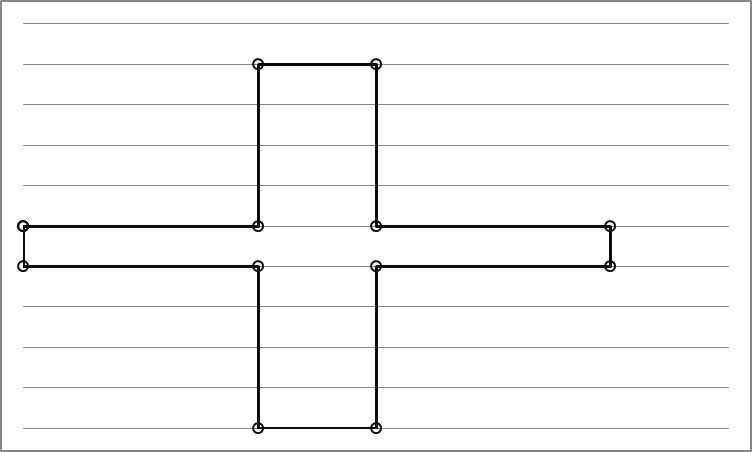
\includegraphics[width=\partitioncomparisionfig\linewidth]{..//Common/images/Pluss.png}} &
\raisebox{\partitioncomparisionraise\height}{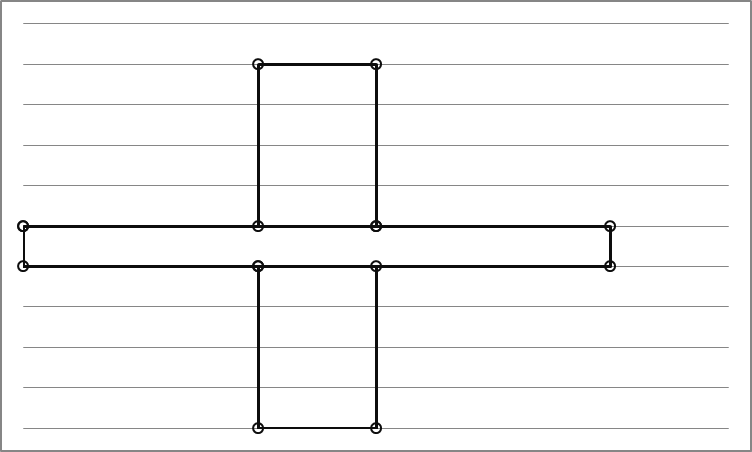
\includegraphics[width=\partitioncomparisionfig\linewidth]{..//Common/images/Plusp.png}}&
\raisebox{\partitioncomparisionraise\height}{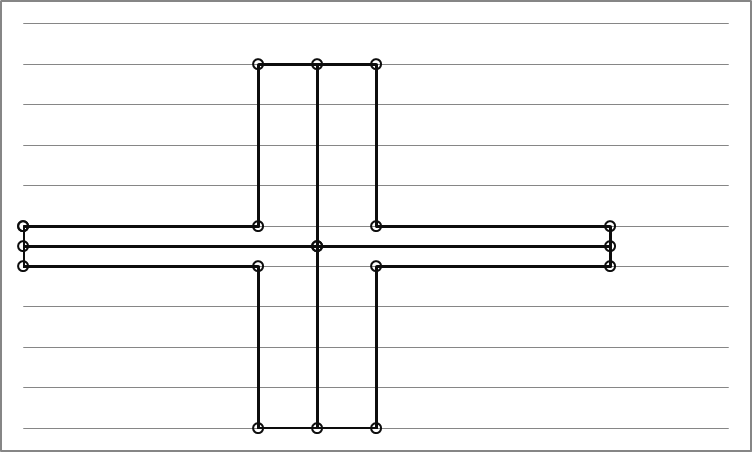
\includegraphics[width=\partitioncomparisionfig\linewidth]{..//Common/images/Plusm.png}} \\

%------------------------------------------------------------------------------------------------------------------------------------
%T &
\raisebox{\partitioncomparisionraise\height}{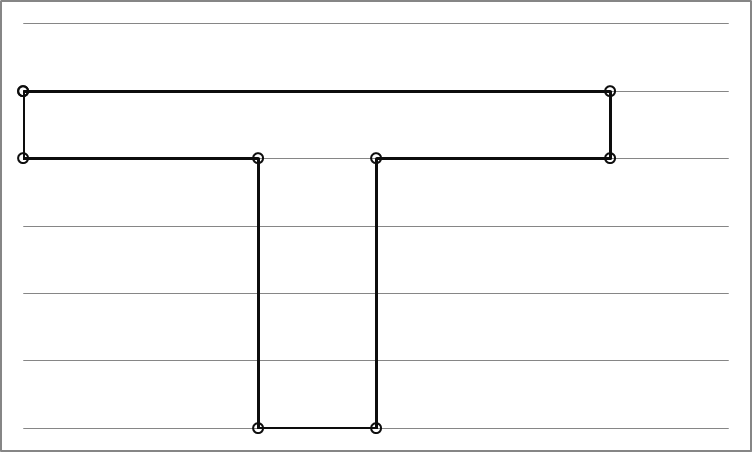
\includegraphics[width=\partitioncomparisionfig\linewidth]{..//Common/images/Ts.png}} &
\raisebox{\partitioncomparisionraise\height}{\includegraphics[width=\partitioncomparisionfig\linewidth]{..//Common/images/Tp.png}}&
\raisebox{\partitioncomparisionraise\height}{\includegraphics[width=\partitioncomparisionfig\linewidth]{..//Common/images/Tm.png}} \\

%------------------------------------------------------------------------------------------------------------------------------------
%K  &
\raisebox{\partitioncomparisionraise\height}{\includegraphics[width=\partitioncomparisionfig\linewidth]{..//Common/images/Ks.png}} &
\raisebox{\partitioncomparisionraise\height}{\includegraphics[width=\partitioncomparisionfig\linewidth]{..//Common/images/Kp.png}}&
\raisebox{\partitioncomparisionraise\height}{\includegraphics[width=\partitioncomparisionfig\linewidth]{..//Common/images/Km.png}} \\

%------------------------------------------------------------------------------------------------------------------------------------
%X &
\raisebox{\partitioncomparisionraise\height}{\includegraphics[width=\partitioncomparisionfig\linewidth]{..//Common/images/Xs.png}} &
\raisebox{\partitioncomparisionraise\height}{\includegraphics[width=\partitioncomparisionfig\linewidth]{..//Common/images/Xp.png}}&
\raisebox{\partitioncomparisionraise\height}{\includegraphics[width=\partitioncomparisionfig\linewidth]{..//Common/images/Xm.png}} \\

%------------------------------------------------------------------------------------------------------------------------------------
%V &
\raisebox{\partitioncomparisionraise\height}{\includegraphics[width=\partitioncomparisionfig\linewidth]{..//Common/images/Vs.png}} &
\raisebox{\partitioncomparisionraise\height}{\includegraphics[width=\partitioncomparisionfig\linewidth]{..//Common/images/Vp.png}}&
\raisebox{\partitioncomparisionraise\height}{\includegraphics[width=\partitioncomparisionfig\linewidth]{..//Common/images/Vm.png}} \\

%------------------------------------------------------------------------------------------------------------------------------------
%Y &
\raisebox{\partitioncomparisionraise\height}{\includegraphics[width=\partitioncomparisionfig\linewidth]{..//Common/images/Ys.png}} &
\raisebox{\partitioncomparisionraise\height}{\includegraphics[width=\partitioncomparisionfig\linewidth]{..//Common/images/Yp.png}}&
\raisebox{\partitioncomparisionraise\height}{\includegraphics[width=\partitioncomparisionfig\linewidth]{..//Common/images/Ym.png}} \\

%\bottomrule
\end{tabular}
\end{table}

\bigskip

%\added[remark={MAT can produce centrelines for such geometries with ease. The authors have not discussed test cases where their method could fail i.e. degenerate geometry.}]
%{In practical scenarios, input geometry may not be clean, can have degeneracies etc, which need to be addressed-corrected before given algorithms to have predictable output. In special situation s like sudden change in thickness (\cite{Sheen2010}) limitations of Polygon Decomposition (Algorithm \ref{alg:midcurves:polygondecomposition}) show up in Midcurves (Algorithm \ref{alg:midcurves:midcurvescreation}). As shown below, although the partitioning is valid, it does not compute Midcurve as expected (even though there could be no clear expectation in this case, as well).}
%
%\begin{itemize}
%[noitemsep,topsep=2pt,parsep=2pt,partopsep=2pt,leftmargin=*]
%\item \textbf{Stepped Component}: There are conflicting expectation from such shape. If it has to mimic the profile then the Midcurve should have the {\em step}. But having a sudden change is sometimes not desirable, so a smooth blended curve could be the correct output.
%
%\raisebox{-.9\height}{\includegraphics[width=0.3\linewidth]{..//Common/images/steps.png}} 
%
%\item \textbf{Partitioning}: The {\em reflex} vertex finds opposite corner to form partitioning chord. 
%
%\raisebox{-.9\height}{\includegraphics[width=0.3\linewidth]{..//Common/images/stepp.png}}
%
%\item As Midcurves from both sides of the chord are to meet together, they are generated in (wrong) opposite direction.
%
%  \raisebox{-.9\height}{\includegraphics[width=0.3\linewidth]{..//Common/images/stepm.png}} 
%\end{itemize}
%
%\begin{table}[!h]
%\caption{Limitations}
%\begin{tabular}[h]{@{} p{0.31\linewidth} p{0.31\linewidth} p{0.31\linewidth}@{}}
%\toprule
%{\bf Shape} & {\bf Partitions} & {\bf Midcurves}\\
%\midrule
%\raisebox{-.9\height}{\includegraphics[scale=0.27]{..//Common/images/steps.png}} &
%\raisebox{-.9\height}{\includegraphics[scale=0.27]{..//Common/images/stepp.png}}&
%\raisebox{-.9\height}{\includegraphics[scale=0.27]{..//Common/images/stepm.png}} \\
%\bottomrule
%\end{tabular}
%\label{table_limitations}
%\end{table}

%%\subsubsubsection{Limitations of Present Approach}

%%In practical scenarios present challenging situations not dealt with so far. So, here are some of the limitations of the proposed approach:
%%
%%\begin{itemize}
%%[noitemsep,topsep=2pt,parsep=2pt,partopsep=2pt,leftmargin=*]
%%\item \textbf{Facet-ting}: Even if the input is made up of curves, it is faceted to convert to a polygon. This approximation approximates output as well and thus, does not give true Midcurve. It is possible to fit a curve through points of the Midcurve-segments, but it may or may not match the expected result.
%%\item \textbf{Holes}: Input to the algorithm is in the form of single ordered list of vertices, making a non-self-intersecting closed polygon.
%%
%%\raisebox{-.9\height}{\includegraphics[width=0.22\linewidth]{..//Common/images/ProfileHoles.pdf}} 
%%
%%\vspace{2mm}
%%
%%In case of holes, a connecting line is added to reach to internal holes to form a path, which does not traverse the given segments twice. If the number of holes are more, the situation becomes challenging to find the right connecting chords.
%%\end{itemize}

\subsection{Results and Discussions}

%%Approach presented in this chapter has been applied not just to the relevant ``thin-walled'' profiles but also to some typical real-life shapes. %(Table \ref{table_PracticalMidcurves}) . 
Following are some of the examples taken from academic papers for benchmarking midcurve output against the proposed approach.

\def\resultscasestablewidth{0.4}
%
%\begin{table}[htb]
%\caption{Medials of real-life shapes}
%\begin{tabular}[htb]{@{}p{0.45\linewidth} p{0.3\linewidth}@{}}
%\toprule
%{\bf Type } & {\bf Midcurves}\\
%\midrule

\begin{enumerate}
[noitemsep,topsep=2pt,parsep=2pt,partopsep=2pt,leftmargin=*]

\item
%------------------------------------------------------------------------------------------------------------------------------------
Glass profile was presented by Fischer et. al~\cite{Elber1999}. 

%%\bigskip

\begin{figure}[h!]
\centering     %%% not \center
\subfloat[Loop Elimination (Source: Fischer~\cite{Elber1999})]{\label{fig_fischerglass}\includegraphics[width=0.6\linewidth]{../Common/images/fischerglass}} \quad
\subfloat[Proposed Apporach]{\label{fig_glass}\includegraphics[width=0.23\linewidth]{../Common/images/Glassmc}} \quad
\caption{Midcurve of a Glass Profile}
  \label{fig:midsurfcelljoin:Glassmc}
\end{figure}

%%\bigskip

Figure~\ref{fig_fischerglass} shows an erroneous loop which had to be eliminated in the post-processing. No such post-processing is needed in the proposed approach and the output as seen in Figure~\ref{fig_glass} is appropriate. This example has been particularly chosen for showcasing midcurve of a profile, having free-form curves and variable thickness.

%\item
%%------------------------------------------------------------------------------------------------------------------------------------
%Profile presented by Ramanathan~\cite{Ramanathan2004}. %&
%
%\vspace{1mm}
%
%\includegraphics[width=\resultscasestablewidth\linewidth]{..//Common/images/DoubleKmc.png}%\\
%

\item
%------------------------------------------------------------------------------------------------------------------------------------
Pinto's~\cite{Pinto2009} example of planar polygonal Horse profile. 


%%\bigskip

\begin{figure}[h!]
\centering     %%% not \center
\subfloat[Erroneous Extra Branches (Source: Pinto~\cite{Pinto2009})]{\label{fig_pinto}\includegraphics[width=0.4\linewidth]{../Common/images/pinto_1.pdf}} \quad
\subfloat[Proposed Approach]{\label{fig_Horsemc}\includegraphics[width=0.5\linewidth]{../Common/images/Horsemc}} \quad
\caption{Midcurve of a Free Form Profile}
  \label{fig:midsurfcelljoin:Horsemc}
\end{figure}

%%\bigskip

Figure~\ref{fig_pinto} shows the midcurve (MAT) computed by Pinto's ~\cite{Pinto2009} approach whereas  Figure~\ref{fig_Horsemc} shows output by the proposed approach. It can be noted that all the erroneous branches at the corners have been eliminated. %&


\item
%------------------------------------------------------------------------------------------------------------------------------------
Woo~\cite{Woo2013} presented following example to demonstrate appropriate extensions. 

%%\bigskip

\begin{figure}[h!]
\centering     %%% not \center
\subfloat[Erroneous Patch (Source: Woo~\cite{Woo2013})]{\label{fig_wooext}\includegraphics[width=0.43\linewidth]{../Common/images/wooext.pdf}} \quad
\subfloat[Proposed Approach]{\label{fig_Woomc}\includegraphics[width=0.5\linewidth]{../Common/images/Woomc}} \quad
\caption{Midcurve Extensions}
  \label{fig:midsurfcelljoin:Woomc}
\end{figure}

%%\bigskip

Figure~\ref{fig_wooext} is output of the traditional face pairing approach. Woo had to devise a logic to get rid off the invalid pairs creating such extensions. When mapped to 2D profile domain, it would result in an erroneous segment, as seen in the circle. Figure~\ref{fig_Woomc} shows the correct output by proposed method.


%\bottomrule
%
%\end{tabular}
%\label{table_PracticalMidcurves}
%\end{table}
\end{enumerate}

%\begin{itemize}[noitemsep,topsep=2pt,parsep=2pt,partopsep=2pt,label={},leftmargin=*]
%\begin{itemize}
%
%\item Glass profile was presented by Fischer~\cite{Elber1999}. They had to carry-out loop-elimination step to eliminate the self-intersection that occurred after the first offset-like operation.
%
%\includegraphics[angle=90, width=\linewidth]{..//Common/images/Glassmc.png}
%
% Such post-processing is not required in the approach presented here.
%
%%------------------------------------------------------------------------------------------------------------------------------------
%\item Double K profile presented by Ramanathan~\cite{Ramanathan2004}.
%
%\includegraphics[width=\linewidth]{..//Common/images/DoubleKmc.png}
%
%%------------------------------------------------------------------------------------------------------------------------------------
%\item  Pinto's~\cite{Pinto2009} example of planar polygonal Horse profile. All the branches at the corners have been eliminated.
%
%\includegraphics[width=\linewidth]{..//Common/images/Horsemc.png}
%
%%------------------------------------------------------------------------------------------------------------------------------------
%\item Sheen et al~\cite{Sheen2010} took  typical plastic injection part profile. Approach presented here does not need any additional split operations.
%
%\includegraphics[width=\linewidth]{..//Common/images/Sheen1mc.png}
%
%They took following profile to compare Midsurface creation in two commercial CAD software packages.  Both produced incorrect results. 
%
%\includegraphics[width=\linewidth]{..//Common/images/Sheen2mc.png}
%
%%------------------------------------------------------------------------------------------------------------------------------------
%\item  Woo~\cite{Woo2013}  presented following example to demonstrate when extensions are appropriate. Extension of midcurves of the first vertical bar up-to boundary is invalid whereas of the second vertical bar is valid, as in the second case, corresponding extended part-faces are present.
%
%\includegraphics[width=\linewidth]{..//Common/images/Woomc.png}
%
%\end{itemize}

%
%\begin{table}[htb]
%\caption{Medials of real-life shapes}
%\begin{tabular}[htb]{@{}p{0.15\linewidth} p{0.75\linewidth}@{}}
%\toprule
%{\bf Type } & {\bf Midcurves}\\
%\midrule
%%------------------------------------------------------------------------------------------------------------------------------------
%Glass profile~\cite{Elber1999} &
%%\raisebox{-.9\height}{\includegraphics[width=1.2\linewidth]{..//Common/images/Glasss.png}} &
%%\raisebox{-.9\height}{\includegraphics[width=0.98\linewidth]{..//Common/images/Glassp.png}}&
%\raisebox{-.9\height}{\includegraphics[width=\linewidth]{..//Common/images/Glassmc.png}} \\
%
%%------------------------------------------------------------------------------------------------------------------------------------
%Double K profile~\cite{Ramanathan2004} &
%%\raisebox{-.9\height}{\includegraphics[width=1.2\linewidth]{..//Common/images/Glasss.png}} &
%%\raisebox{-.9\height}{\includegraphics[width=0.98\linewidth]{..//Common/images/Glassp.png}}&
%\raisebox{-.9\height}{\includegraphics[width=\linewidth]{..//Common/images/DoubleKmc.png}} \\
%
%%------------------------------------------------------------------------------------------------------------------------------------
%Horse profile ~\cite{Pinto2009} &
%%\raisebox{-.9\height}{\includegraphics[width=1.2\linewidth]{..//Common/images/Horses.png}} &
%%\raisebox{-.9\height}{\includegraphics[width=0.98\linewidth]{..//Common/images/Horsep.png}}&
%\raisebox{-.9\height}{\includegraphics[width=\linewidth]{..//Common/images/Horsemc.png}} \\
%
%%------------------------------------------------------------------------------------------------------------------------------------
%Cover Part profile ~\cite{Sheen2010} &
%%\raisebox{-.9\height}{\includegraphics[width=1.2\linewidth]{..//Common/images/Sheen1.png}} &
%%\raisebox{-.9\height}{\includegraphics[width=0.98\linewidth]{..//Common/images/Sheen1.png}}&
%\raisebox{-.9\height}{\includegraphics[width=\linewidth]{..//Common/images/Sheen1mc.png}} \\
%
%%------------------------------------------------------------------------------------------------------------------------------------
%Channel profile ~\cite{Sheen2010} &
%%\raisebox{-.9\height}{\includegraphics[width=1.2\linewidth]{..//Common/images/Sheen1.png}} &
%%\raisebox{-.9\height}{\includegraphics[width=0.98\linewidth]{..//Common/images/Sheen1.png}}&
%\raisebox{-.9\height}{\includegraphics[width=\linewidth]{..//Common/images/Sheen2mc.png}} \\
%
%%------------------------------------------------------------------------------------------------------------------------------------
%Thick Thin profile ~\cite{Woo2013} &
%%\raisebox{-.9\height}{\includegraphics[width=1.2\linewidth]{..//Common/images/Sheen1.png}} &
%%\raisebox{-.9\height}{\includegraphics[width=0.98\linewidth]{..//Common/images/Sheen1.png}}&
%\raisebox{-.9\height}{\includegraphics[width=\linewidth]{..//Common/images/Woomc.png}} \\
%
%%------------------------------------------------------------------------------------------------------------------------------------
%%Cross Channel profile &
%%%\raisebox{-.9\height}{\includegraphics[width=1.2\linewidth]{..//Common/images/Crosss.png}} &
%%%\raisebox{-.9\height}{\includegraphics[width=0.98\linewidth]{..//Common/images/Crossp.png}}&
%%\raisebox{-.9\height}{\includegraphics[width=\linewidth]{..//Common/images/Crossmc.png}} \\
%
%
%\bottomrule
%
%\end{tabular}
%\label{table_PracticalMidcurves}
%\end{table}
